
La primera targeta bancària generalment s'atribueix a la targeta Diners Club, que va ser creada el 1950 en EEUU. La idea darrere de la targeta Diners Club era proporcionar als clients una forma convenient de pagar a restaurants sense necessitat de portar efectiu.

\begin{figure}[h]
    \centering
    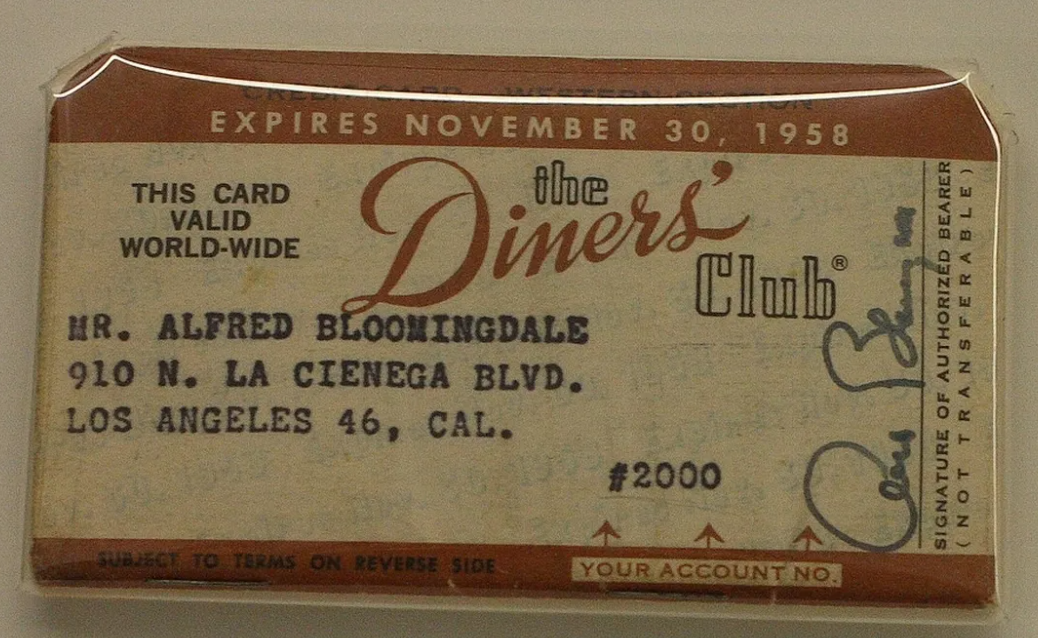
\includegraphics[width=5cm]{primeratarjeta.png}
    \caption{Primera tarjeta de pagament}
\end{figure}  


La targeta Diners Club va ser un precursor important de les targetes de crèdit modernes, i el seu èxit va inspirar la creació daltres targetes bancàries en els anys següents. Poc després, el 1958, es va llançar la targeta American Express, seguida per la introducció de targetes Visa i MasterCard als anys 1960.


L'abril del 1971 es llança la primera targeta bancària a Espanya per part del Banc de Bilbao. En aliança amb BankAmericard, aquesta primera targeta de crèdit permetia el pagament total a final de mes.
\begin{figure}[h]
    \centering
    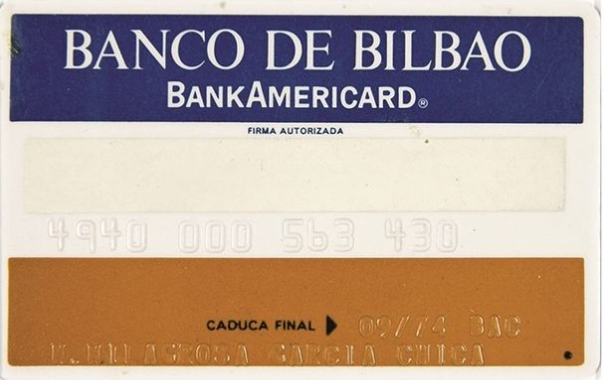
\includegraphics[width=5cm]{primeravisaespanya.png}
    \caption{Primera visa bancaria en Espanya}
\end{figure}  

Les primeres tarjetes funcionaven amb banda magnètica, que conté informació vital, com ara el número de compte i la informació del compte del titular. Quan la targeta llisca o s'insereix en un terminal de pagament, la banda magnètica transfereix aquesta informació al sistema de processament de pagaments, les quals poden ser fàcilment robats i clonats. És important destacar que encara que la banda magnètica ha estat una tecnologia comuna en targetes durant dècades, es considera menys segura en comparació amb altres tecnologies més recents. Tot i que la banda magnètica encara s'utilitza en moltes targetes, especialment en àrees on la infraestructura de pagaments pot ser més antiga. 
\\
\\
Actualment, moltes targetes incorporen tecnologies més avançades com els xips EMV, que contenen un xip que crea un codi únic per a cada transacció, un que no pot ser clonat i que queda inutilitzat un cop completada la transacció. Les tarjetes de xips EMV ha estat un esforç global per reduir el frau relacionat amb targetes. 


